\chapter{Einleitung}
\label{chap:einleitung}

Durch den technischen Fortschritt in den letzten Jahren hat sich der Einsatz von \emph{Augmented Reality} (AR) und \emph{Virtual Reality} (VR) in verschiedenen Anwendungsbereichen etabliert \parencite{Krevelen2010, Zhao2009, Sharples2008, Jung2008}.
Als Nutzerschnittstelle dienen dienen in vielen Anwendungen Smartphones, da die Sensoren (Kameras, Gyrosensor etc.) nun ausreichen, um einfache AR-/VR-Inhalte zu präsentieren \parencite{Li2017b,Feng2017,Yoo2015,Mulloni2012}.
Neben Smartphones ermöglichen Head-Mounted Displays (HMDs) die Anzeige von \emph{Mixed-Reality-} (MR) und VR-Inhalten.
Beispielsweise sind hier die \emph{Microsoft HoloLens} \parencite{Microsoft2018} als AR-HMD oder die \emph{Oculus Rift} \parencite{Facebook2018} und \emph{HTC Vive} \parencite{HTCCorporation2018} als VR-HMD zu nennen (siehe \autoref{fig:devices}).
\begin{figure}[hb]
    \centering
    %\imagebox{%
    \begin{minipage}{0.3\textwidth}
        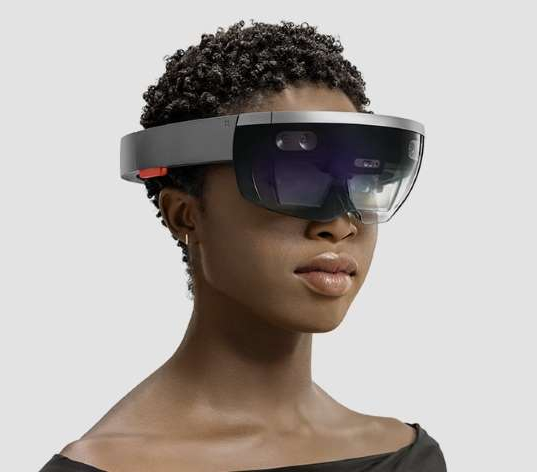
\includegraphics[width=.9\linewidth]{figures/Microsoft2018_HoloLens_worn}
    \end{minipage}%
    \hfill
    \begin{minipage}{0.45\textwidth}
        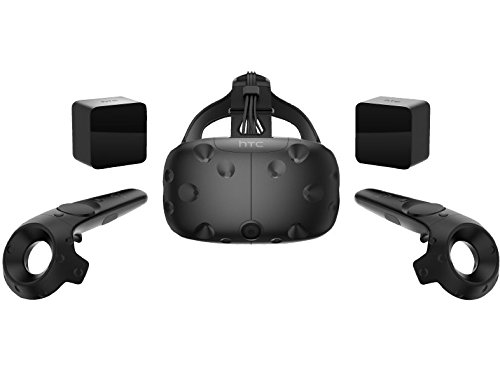
\includegraphics[width=.9\linewidth]{figures/htc_vive}
    \end{minipage}%
    \hfill
    \begin{minipage}{0.25\textwidth}
        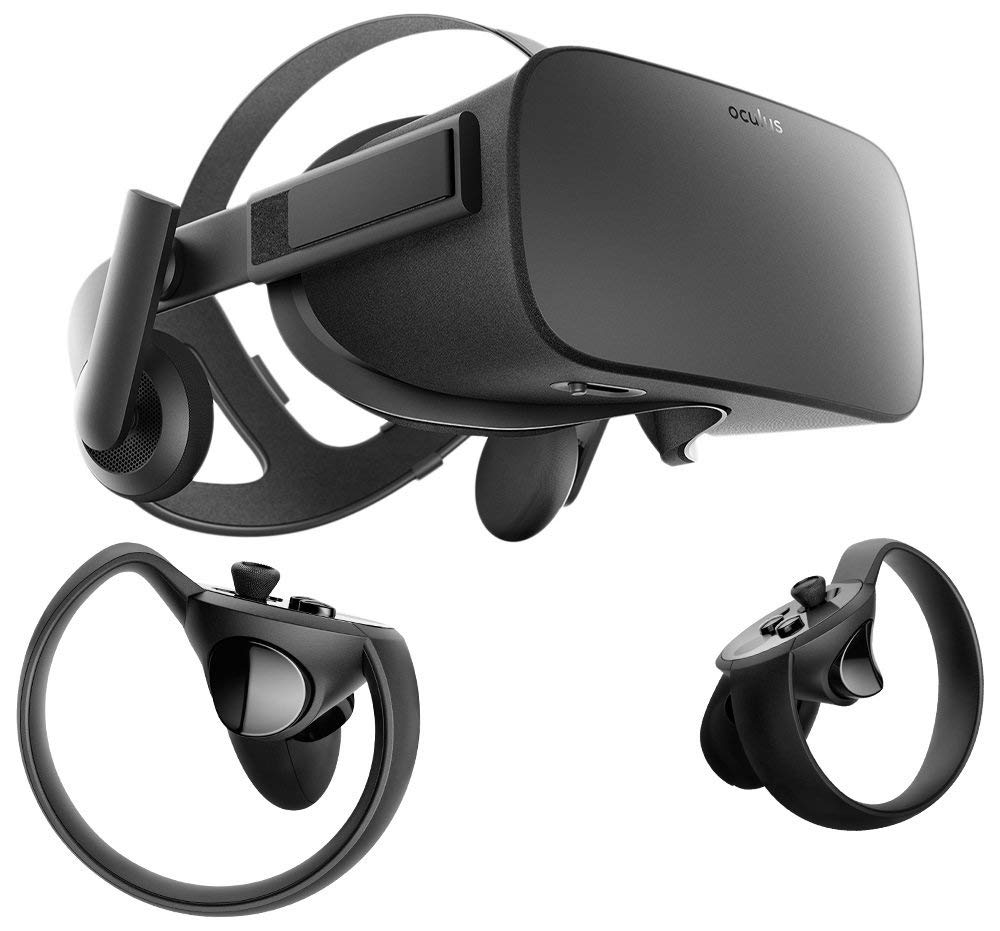
\includegraphics[width=.9\linewidth]{figures/oculus_rift}
    \end{minipage}%
    %}
    \caption{Diverse MR- und VR-HMDs. Microsoft HoloLens (Links), HTC Vive (Mitte) und Oculus Rift (Rechts). \quelle{\cite{Microsoft2018, Amazon2018b, Amazon2018}}}
    \label{fig:devices}
\end{figure}

Bei AR wird die Grenze zwischen dem Reellen und dem Virtuellen aufgehoben, indem virtuelle Inhalte in Echtzeit mit sechs Freiheitsgraden in die reale Welt überlagert werden.
\autoref{fig:mrtouch} zeigt z.\,B., wie virtuelle Nutzerschnittstellen in die physische Welt platziert werden und über Berührungen gesteuert werden können.
In der Vergangenheit wurde von Forschern AR unter anderem eingesetzt, um räumliche Informationen in der Umgebung von Nutzern anzuzeigen.
Beispielsweise wird die Schritt-für-Schritt-Navigation durch AR unterstützt \parencite{Hoellerer1999, Hashish2017, Mulloni2012} und reales Kartenmaterial mit digitalen Inhalten augmentiert \parencite{Rohs2009, Morrison2009, Reitmayr2005}.
\begin{figure}[ht]
    \centering
    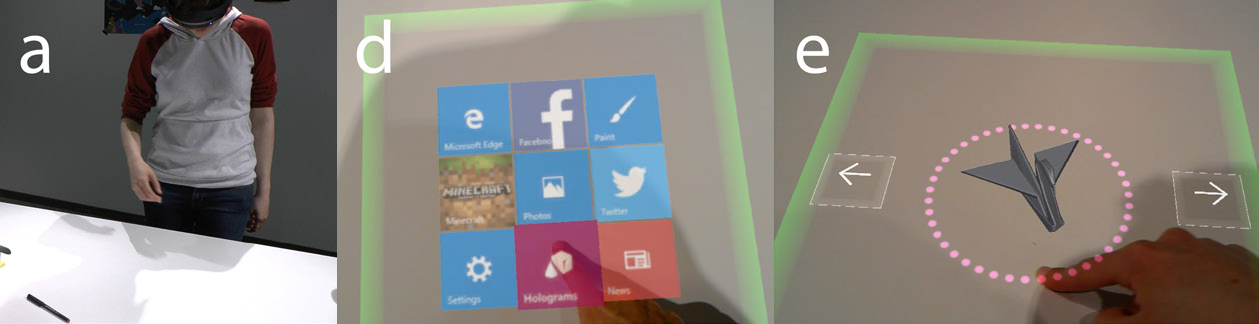
\includegraphics[width=\textwidth]{figures/mrtouch}
    \caption{Virtuelle Nutzeroberflächen werden auf physischen Objekten platziert und mit Berührungsgesten bedient. \quelle{\cite{Xiao2018}}}
    \label{fig:mrtouch}
\end{figure}

\section{Motivation und Ziel der Arbeit}
\label{sec:motivation_ziel}
Das Ziel \emph{dieser} Arbeit ist die Entwicklung einer neuen Herangehensweise, digitale Karten mithilfe eines MR-HMDs in die reale Welt zu integrieren: die \textbf{Megamap}.
Als Megamap wird eine Kartendarstellung definiert, bei der ein dreidimensionales Abbild der Umgebung im verkleinerten Maßstab um den Nutzer herum angezeigt wird.
Der Nutzer steht inmitten der augmentierten Karte und kann sich auf dieser frei bewegen.
Die virtuelle Karte verhält sich somit, als sei sie ein reales Objekt in der Umgebung.

Die ursprüngliche Idee für die Megamap-Darstellung stammt aus dem Spiel \emph{Tom Clancy's The Division} (TCTD) \parencite{Ubisoft2018} (siehe \autoref{fig:megamap}).
Eine Karte der Umgebung (eine Variante von New York) wird mit relevanten Spielobjekten und Ortsnamen als AR-Interface um den Charakter herum angezeigt.
Die Karte erlaubt dem Spieler unter anderem, Wegpunkte festzulegen (Navigation), interessante Punkte in der Umgebung anzuzeigen und zu filtern (Exploration) sowie die Ansicht durch Verschieben und Zoomen der Karte anzupassen.
Ebenso werden Missionsziele, andere Charaktere und Events durch Icons in der Karte hervorgehoben.
All diese Informationen sind vom aktuellen Kontext des Spiels abhängig.
Das heißt, es werden nur Informationen angezeigt die für die aktuelle Situation des Spielers relevant sind.
\begin{figure}[t]
    \centering
    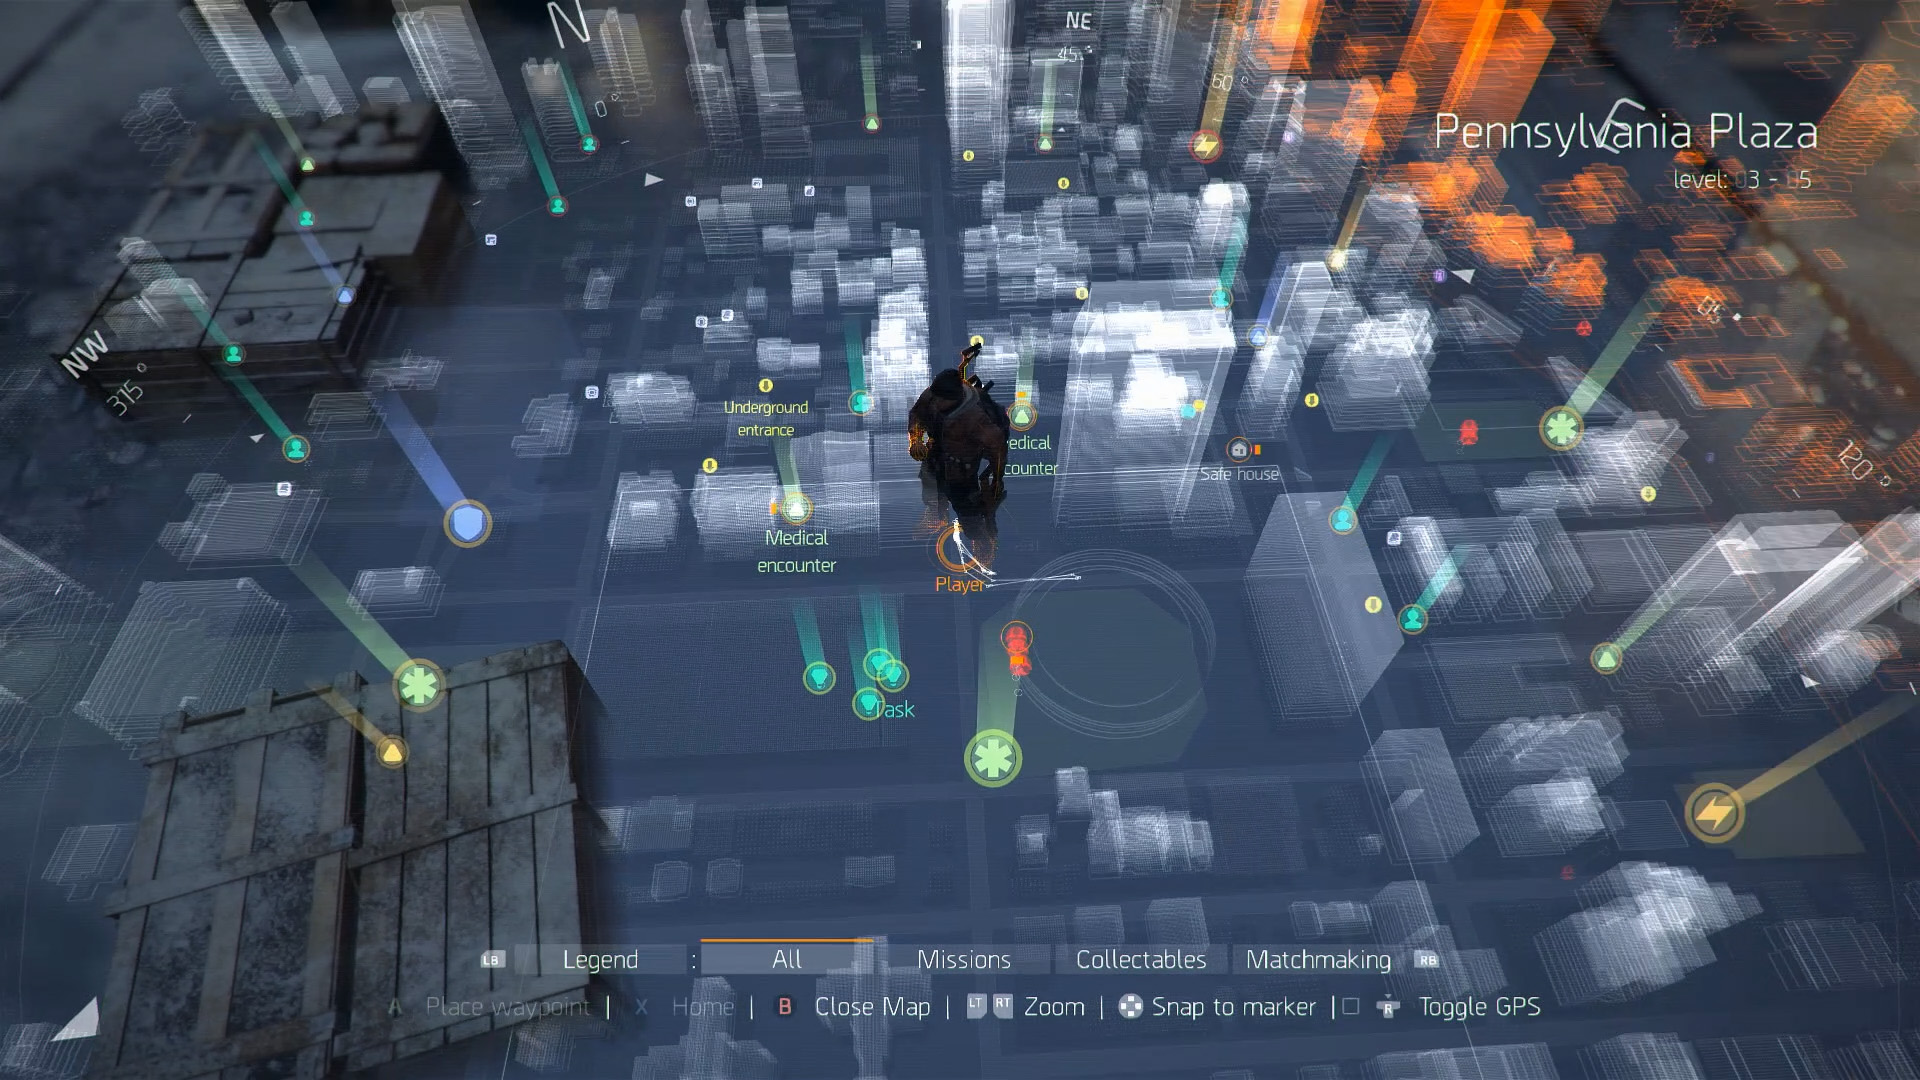
\includegraphics[width=\textwidth]{figures/the_division_megamap.jpg}
    \caption{Die \enquote{Megamap} aus \emph{Tom Clancy's The Division}. Symbole zeigen Missionsziele, Gegenstände und wichtige Orte im Spiel. \quelle{\cite{MYDIVISION.NET2014}}}
    \label{fig:megamap}
\end{figure}

Eine Darstellung von räumlichen Informationen als Megamap bietet gegenüber existierenden Ansätzen einige Vorteile:
\begin{itemize}
    \item Durch die Verwendung des HMDs bleiben die Hände der Nutzer frei. %
    Sie können die Karte nutzen und zeitgleich mit beiden Händen mit der Umgebung interagieren.

    \item Da die Megamap direkt in das Sichtfeld der Nutzer integriert ist, müssen sie die Karte nicht wiederholt mit der Umgebung abgleichen. %
    Dies verbessert die Aufmerksamkeit der Nutzer für ihr Umfeld und reduziert den mentalen Aufwand während der Nutzung \parencite{Bark2014, Narzt2006, Kim2009}.

    \item Die Megamap bewegt sich mit den Nutzern mit. Sie kann daher auch während der Fortbewegung genutzt werden.

    \item Mit der Megamap können sowohl Außen- als auch Innenbereiche (z.\,B. Gebäude) dargestellt werden.
\end{itemize}

Im Rahmen dieser Arbeit wird der Prototyp einer Megamap-Anwendung entwickelt.
Spezifisch zielt die Anwendung auf die Nutzung in Innenbereichen wie Gebäude ab, da bisherige MR-HMDs Probleme mit der Verwendung im Freien aufweisen \parencite{Schroeder2017, Strange2018}.

Da sich außerdem die bisherigen Ansätze mit der Karten\emph{navigation} (\enquote{von A nach B}) beschäftigen, wird in dieser Masterarbeit der Anwendungsfall der Karten\emph{exploration} fokussiert.
Bei der Kartenexploration geht es um die Erkundung von Umgebungen anhand von kontextbasierten Ortsdaten.
Kontextbasierte Ortsdaten sind Daten, die von der aktuellen Situation abhängig sind, wie z.\,B. der aktuellen Position des Nutzers (\textquote{Wo ist das von mir aus nächste Restaurant?}/\textquote{Wieviele Spielplätze sind in meiner Nähe?}).
Ortsdaten können ebenso von der Zeit abhängen (\textquote{Welche Supermärkte in der Gegend sind geöffnet?}).
Übertragen auf die Innenbereichsnutzung stehen mit der Megamap verschiedene explorative Funktionen bereit, beispielsweise das Suchen nach den Büros von Personen oder den Standorten von öffentlichen Druckern.
Nutzer können sich mit der Megamap einen detaillierten Überblick über das Gebäude verschaffen, in dem sie sich befinden.

Als Zielplattform dient das Vive-HMD.
HMDs haben gegenüber Smartphones einige technische Vorteile.
Positionen und Orientierungen der Nutzer sind über Tracking präziser möglich.
MR-HMDs wie die HoloLens oder die \emph{Magic Leap One} \parencite[siehe \autoref{fig:magic_leap}]{MagicLeap2018} verwenden Infrarotkameras, um Strukturen der Umgebung virtuell in Echzeit zu rekonstruieren.
Die reale Umgebung bleibt dank des durchsichtigen Glases weiterhin sichtbar.
Zudem können die Hände für Gesteninteraktionen oder Controller verwendet werden anstatt das Display halten zu müssen.
\begin{figure}[tb]
    \centering
    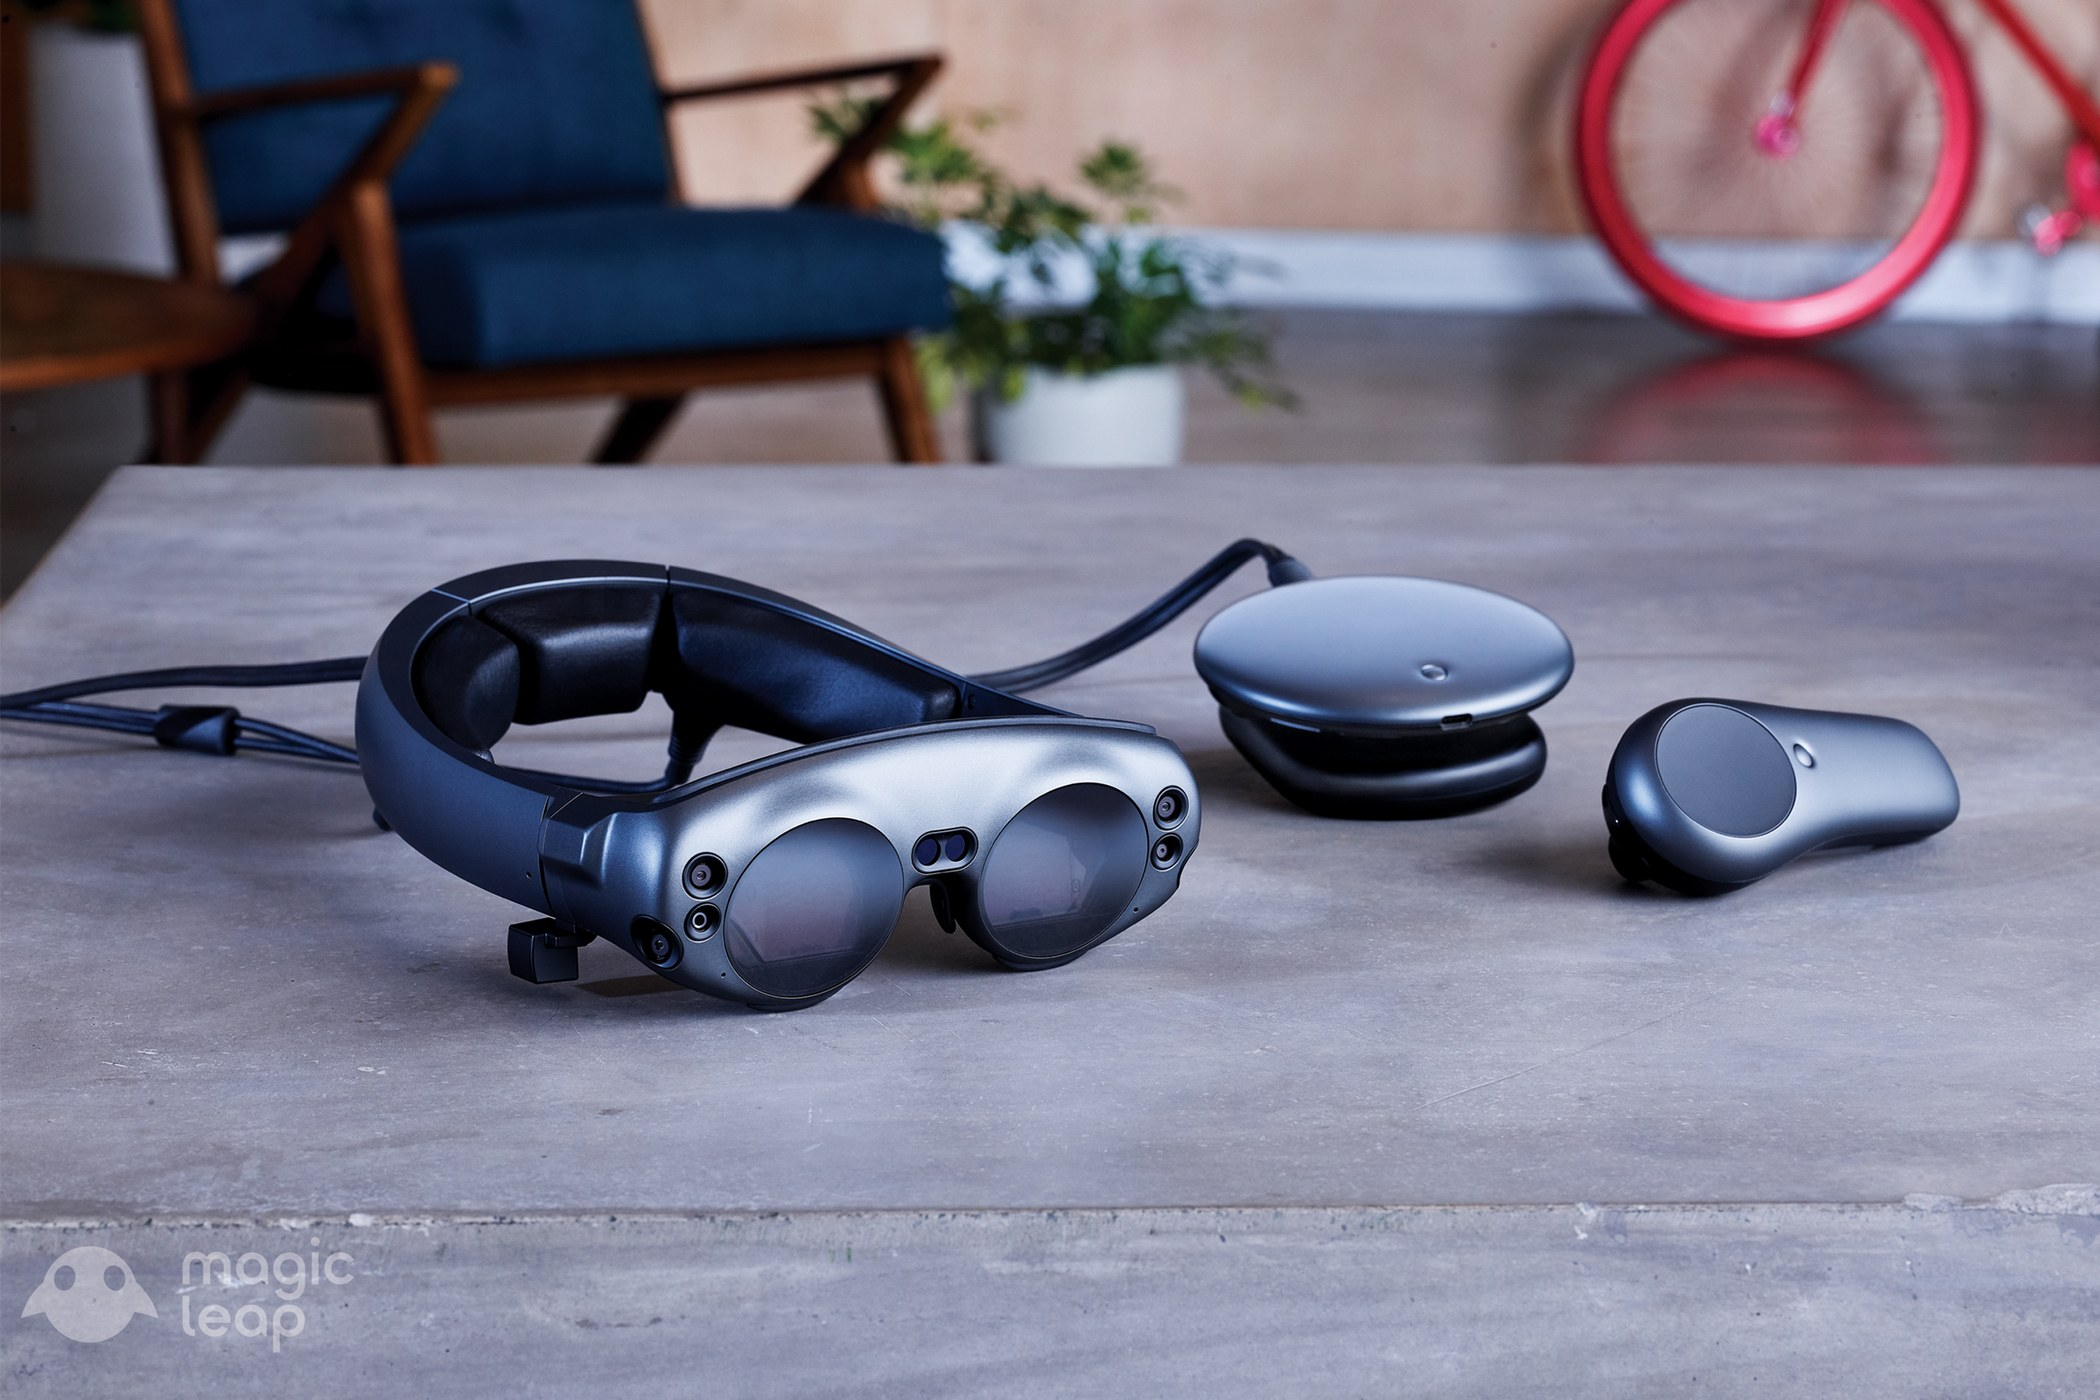
\includegraphics[trim={0, 7cm, 0, 7cm}, clip, width=\textwidth]{figures/magicleap}
    \caption{Das Magic Leap One MR-HMD. \quelle{\cite{MagicLeap2018b}}}
    \label{fig:magic_leap}
\end{figure}

Zu Beginn der Arbeit war das Ziel die Implementierung der Megamap für das Magic Leap One HMD.
Da dieses aber erst im späteren Verlauf der Arbeit als Entwicklervorschau verfügbar war, wurde stattdessen die Implementierung für das Vive-HMD in VR umgesetzt.
Die \enquote{reale} Umgebung des Nutzers wird dabei mit einer virtuellen Nachbildung simuliert.
So lässt sich das grundlegende Megamap-Konzep in zukünftigen Arbeiten auf ein MR-HMD übertragen.

%Die Implementierung der Megamap dient der Beantwortung der zentralen Fragestellung dieser Arbeit:
%\begin{quote}
%    \itshape
%    Ist eine in die Umgebung integrierte 3D-Megamap geeignet, um Nutzer bei der Exploration von Gebäuden zu unterstützen?
%\end{quote}
%Der Prototyp wird daher in einer Nutztungsevaluation getestet, um seine Effektivität für die Gebäudeexploration festzustellen.

%Als Inspirationsquelle für die Anwendung dienen neben bereits existierenden Kartenanwendungen wie Google Maps und Ansätzen aus der Forschung auch digitale Spiele.
%Da in Spielen Aufgaben wie Navigation und Exploration von großer Bedeutung sind, kann hier unterschiedliche Ansätze zur Navigations- und Explorationsunterstützung gefunden werden.
%Dies ist am Beispiel TCTD erkennbar.

Da die Idee für die Megamap einem Videospiel entspringt ist nicht unmittelbar klar, ob sich das Konzept auf die Nutzung in der realen Welt übertragen lässt.
Insbesondere, weil die Megamap aus TCTDs Dritte-Person-Perspektive in die Erste-Person-Perspektive überführt wird.
Die Eignung der Megamap für die Kartenexploration wird daher am entwickelten Prototyp in einer Nutzerstudie überprüft.
Einerseits werden die subjektiven Eindrücke der Probanden von der Nutzung der Megamap festgehalten.
Andererseits wird ihre Effektivität und Effizient mit einer herkömmlichen 2D-Darstellung einer Indoor-Karte verglichen.

\section{Struktur der Arbeit}
\label{sec:struktur}
Die restliche Arbeit ist in die folgenden Abschnitte unterteilt:

\noindent
Im nächsten Kapitel wird der Stand der Forschung und Technik zur Darstellung von dreidimensionalen Karten beleuchtet.
Die Unterschiede zum Konzept dieser Arbeit sowie deren Beitrag zum Thema werden ebenso herausgearbeitet.
\autoref{chap:concept} geht detailliert auf die Konzeptionierung der 3D-Megamap ein.
Es wird vor allem beschrieben, welche Interaktionen für die Kartenexploration wichtig sind und wie diese in der Megamap-Anwendung umgesetzt werden sollen.
Danach wird in \autoref{chap:implementation} die Implementierung des konkreten Prototyps beschrieben.
\autoref{chap:evaluation} präsentiert die Durchführung der Nutzerevaluation der Anwendung sowie deren Ergebnisse.
Schließlich werden in \autoref{chap:closing} offene Fragen und Probleme dieser Arbeit genannt, welche für zukünftige Arbeiten von Interesse sind.
%
\cleardoublepage
